\section{Explicit Euler Method}

\begin{minted}[frame=lines,framerule=3pt, framesep=10pt, fontsize=\small, linenos]{matlab}
% Initialization
f=@(t,y) exp(-t);

a=3;      b=12;
n=10;     h=(b-a)/n;    t=a:h:b;

y(1)=2;   % Inital guess

% Scheme
for i=1:n
  y(i+1)=y(i)+h*f(t(i),y(i));

  fprintf('Solution at t=%d is %f.\n',t(i+1),y(i+1));
end

% Graph
plot(t,y,'-b*');
xlabel('time');   ylabel('distance');
title('Numerical solution by Explict Euler method');
\end{minted}

\begin{figure}[h]
  \centering
  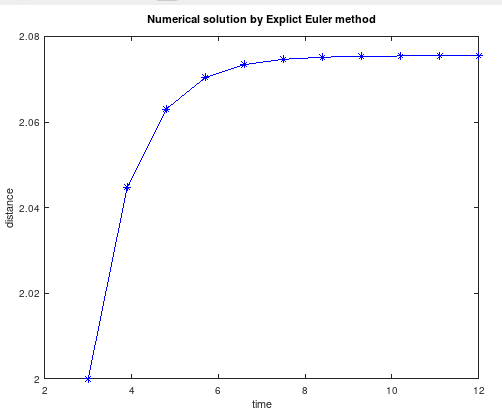
\includegraphics[width=11cm, height=6.5cm]{euler.png}
\end{figure}

\vspace{9mm}

\section{Implicit Euler Method}

\begin{minted}[frame=lines,framerule=3pt, framesep=10pt, fontsize=\small, linenos]{matlab}
% Initialization
f=@(t,y) exp(-t);

a=3;      b=12;
n=10;     h=(b-a)/n;    t=a:h:b;

y(1)=2;   % Inital guess

% Scheme
for i=1:n
  k(i)=f(t(i),y(i));
  y(i+1)=y(i)+h*f(t(i+1),y(i)+h*k(i));

  fprintf('Solution at t=%d is %f.\n',t(i+1),y(i+1));
end

% Graph
plot(t,y,'-b*');
xlabel('time');   ylabel('distance');
title('Numerical solution by Implict Euler method');
\end{minted}
\clearpage

\section{Second order Runge-Kutta method}

\begin{minted}[frame=lines,framerule=3pt, framesep=10pt, fontsize=\small, linenos]{matlab}
% Initialization
f=@(t,y) exp(-t);

a=3;      b=12;
n=10;     h=(b-a)/n;    t=a:h:b;

y(1)=2;   % Inital guess

% Scheme
for i=1:n
  k(i)=f(t(i),y(i));
  k(i+1)=f(t(i+1),y(i)+h*k(i));

  y(i+1)=y(i)+0.5*h*(k(i)+k(i+1));

  fprintf('Solution at t=%d is %f.\n',t(i+1),y(i+1));
end

% Graph
plot(t,y,'-b*');
xlabel('time');   ylabel('distance');
title('Second order Runge-Kutta method');

\end{minted}
\clearpage

\section{Fourth order Runge-Kutta Method}

\begin{minted}[frame=lines,framerule=3pt, framesep=10pt, fontsize=\small, linenos]{matlab}
% Initialization
f=@(t,y) exp(-t);

a=3;      b=12;
n=10;     h=(b-a)/n;    t=a:h:b;

y(1)=2;   % Inital guess

% Scheme
for i=1:n
  k(i)=f(t(i),y(i));
  k(i+1)=f(t(i)+h/2,y(i)+h/2*k(i));
  k(i+2)=f(t(i)+h/2,y(i)+h/2*k(i+1));
  k(i+3)=f(t(i)+h,y(i)+h*k(i+2));

  y(i+1)=y(i)+(h/6)*(k(i)+2*k(i+1)+2*k(i+2)+k(i+3));

  fprintf('Solution at t=%d is %f.\n',t(i+1),y(i+1));
end

% Graph
plot(t,y,'-b*');
xlabel('time');   ylabel('distance');
title('Fourth order Runge-Kutta method');
\end{minted}
